% !TEX root = ../main.tex

Im Forschungsfeld der Informationsvisualisierung ist die Wikipedia eine häufig verwendete Datenquelle und stellt aufgrund ihres komplexen Aufbaus und ihrer enormen Größe eine besondere Herausforderung in diesem Bereich dar.\\
In der Arbeit von Holloway~\cite{holloway2007analyzing} wird die inhaltliche Reichweite der Wikipedia in Form einer \emph{Category Map} dargestellt.
Dafür werden genau diejenigen Kategorien durch eine Kante miteinander verbunden, die mindestens einen gemeinsamen Artikel haben. Auf Basis dieser neuen Verbindungen wird ein Kategoriengraph gezeichnet.
\begin{figure}[H]
    \centering
    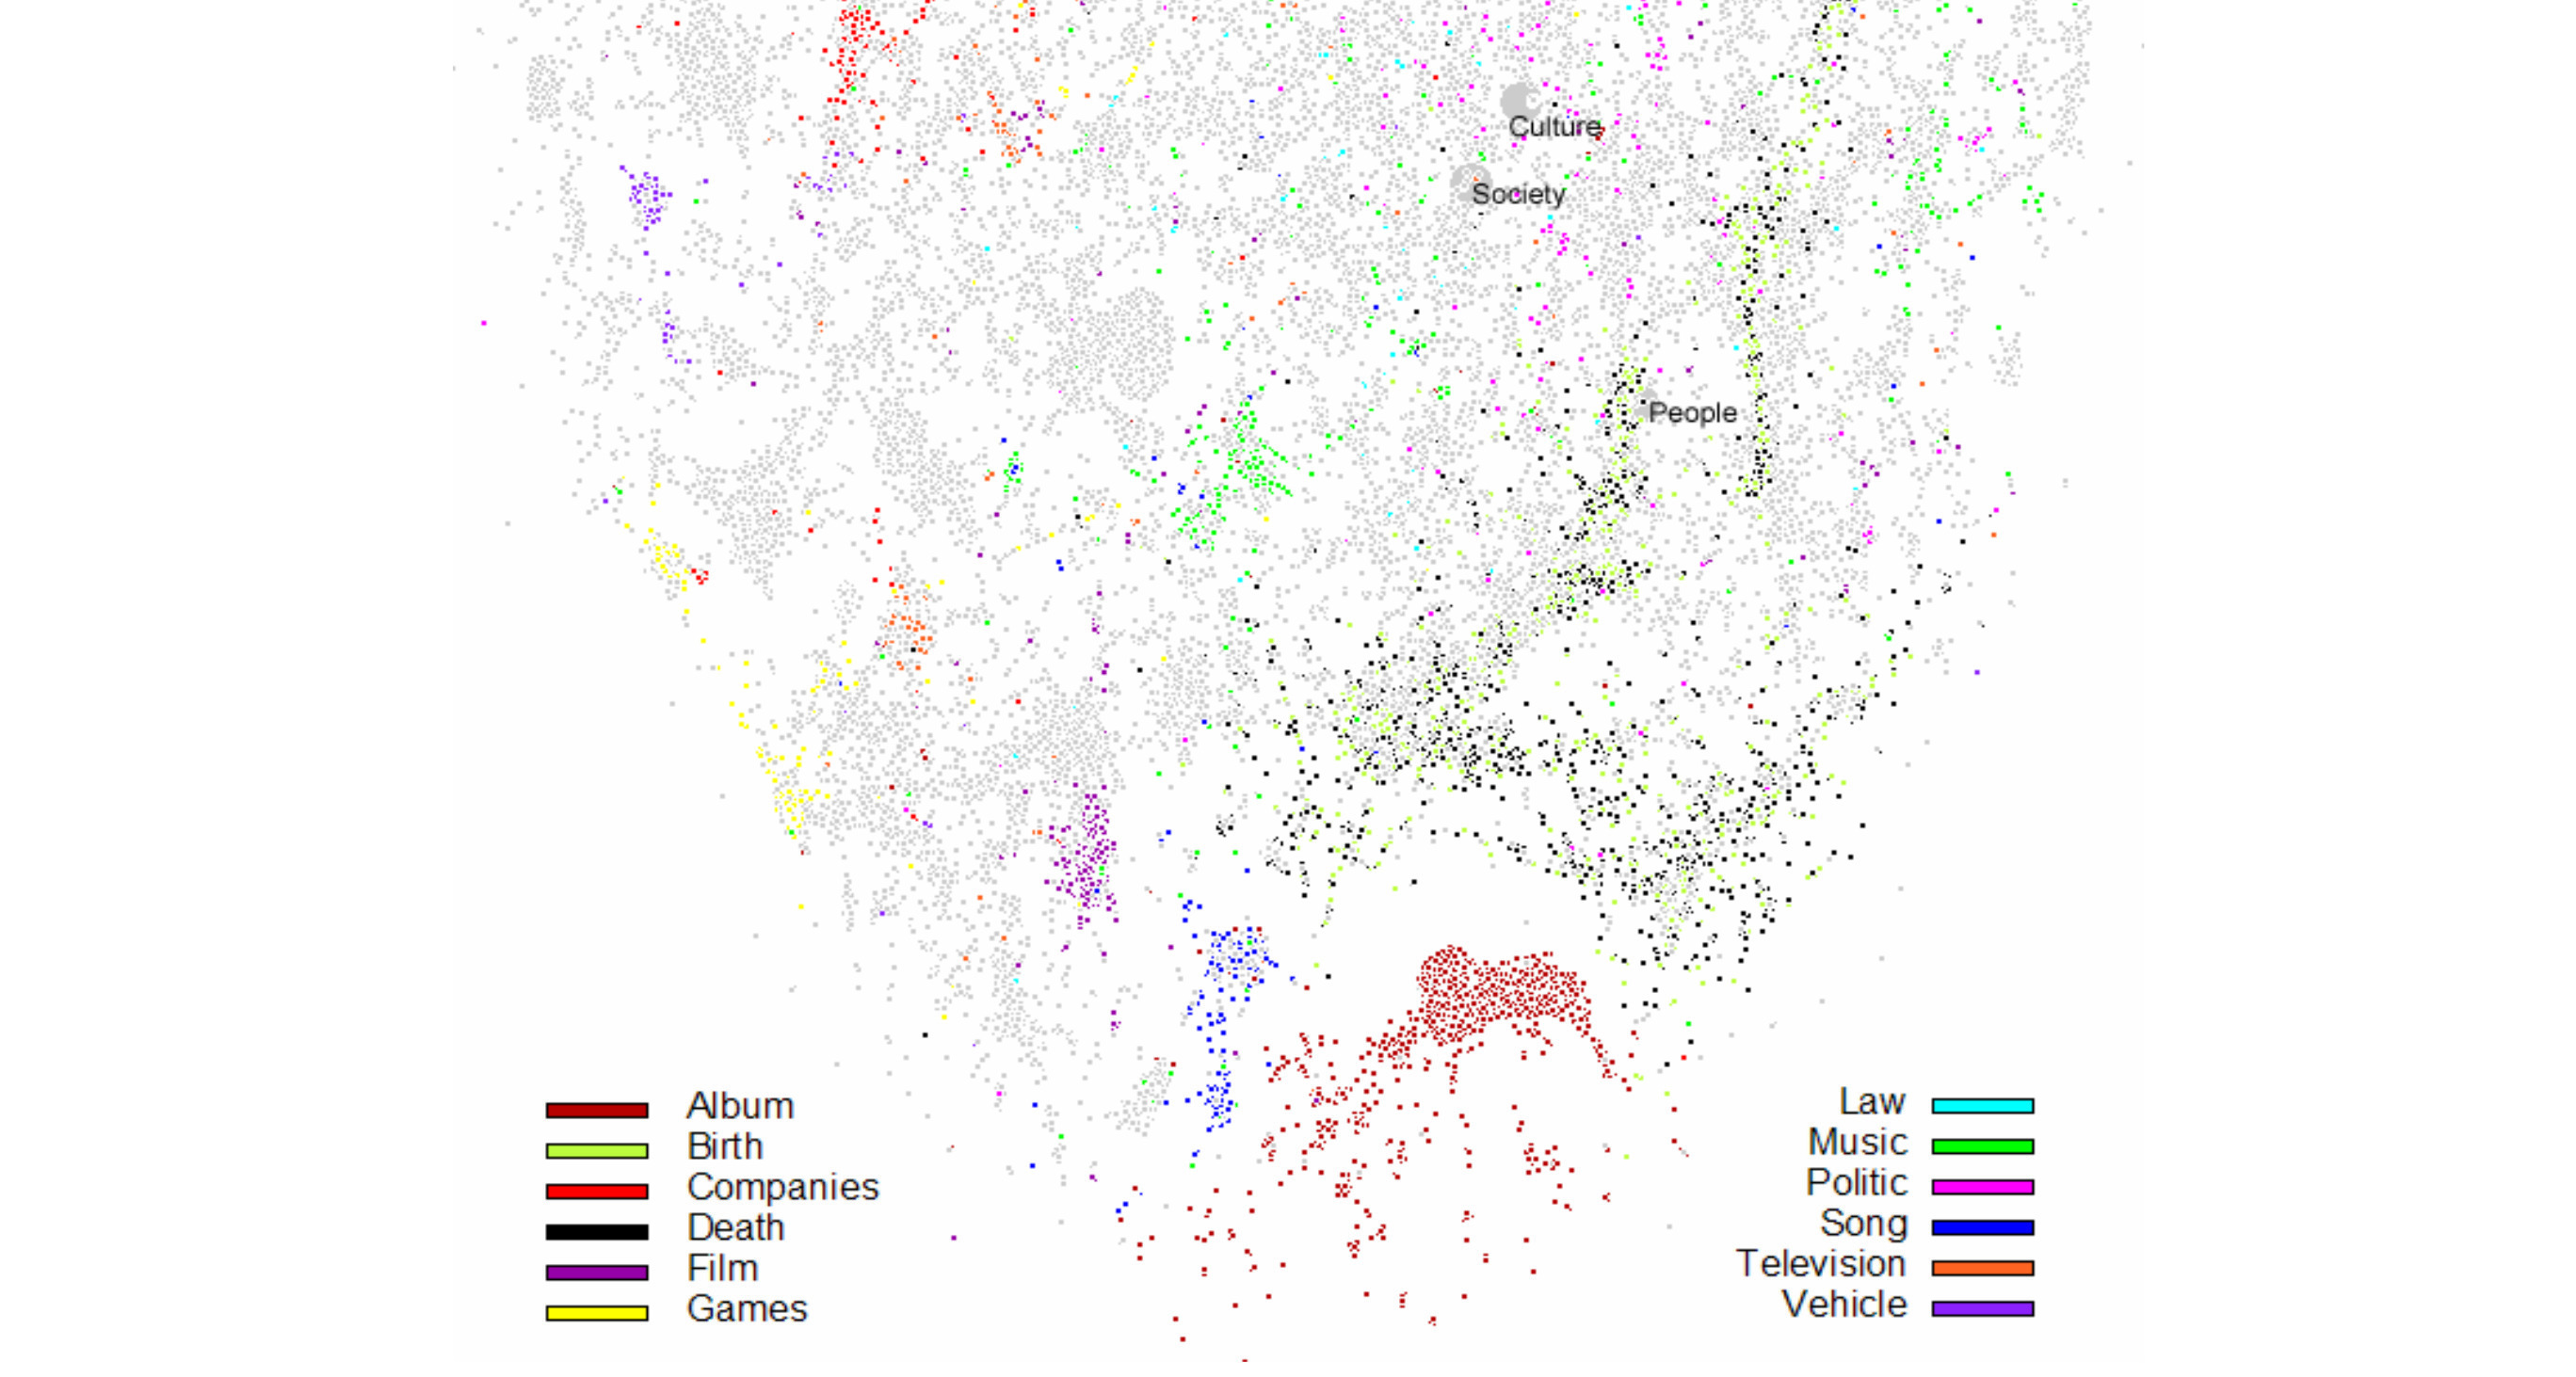
\includegraphics[scale=.14]{images/hol-wikivis3}
    \caption{Karte von Kategorien angeordnet nach der Methodik von Holloway~\cite{holloway2007analyzing}.}
    \label{fig:hol-wikivis}
\end{figure}
Darüber hinaus wird ein Gewicht eingeführt, das die Stärke dieser Verbindungen abbilden soll.
Das Gewicht ist eine Modifikation der Kosinusähnlichkeit.
Um die inhaltliche Reichweite des dargestellten Graphen deutlicher hervorzuheben, werden die \emph{Main Topic Categories} beschriftet und die Kategorien farblich markiert, die in ihrem Titel besonders häufige auftretende Wörter enthalten.
Die Abbildung~\ref{fig:hol-wikivis} zeigt diese \emph{Category Map}.\\
Die Arbeit \emph{Wikiviz: Visualizing Wikipedia}~\cite{harrison2006wikiviz} stellt den Graphen von Verbindungen zwischen Kategorien dar, um ungewöhnliche Verbindungen zwischen Kategorien zu veranschaulichen, wie in der Abbildung~\ref{fig:harr-wikiviz} zu erkennen.
Ausgehend von einer Startkategorie werden die Verbindungen bis zur Tiefe 5 gezeichnet.
Darüber hinaus liegen die Kategorien, die untereinander viele Verbindungen besitzen, näher beieinander als solche, die weniger Verbindungen untereinander aufweisen.

Für die Anordnung der Kategorien entwickelt Harrison in seiner Arbeit eine eigene Methode, da die Ansätze wie \emph{Force-Directed-Layout} nach~\cite{fruchterman1991graph} und~\cite{kamada1989algorithm} zu rechenintensiv sind und sich deshalb die Laufzeit der Algorithmen mit einer steigenden Anzahl an Kategorien verlängert.
Die Informationen über die Verbindungen von Kategorien werden direkt aus den Wikipedia-Seiten extrahiert, da die Daten aus der Wikipedia-Datenbank zu unpräzise sind~\cite{harrison2006wikiviz}.
\begin{figure}[H]
    \centering
    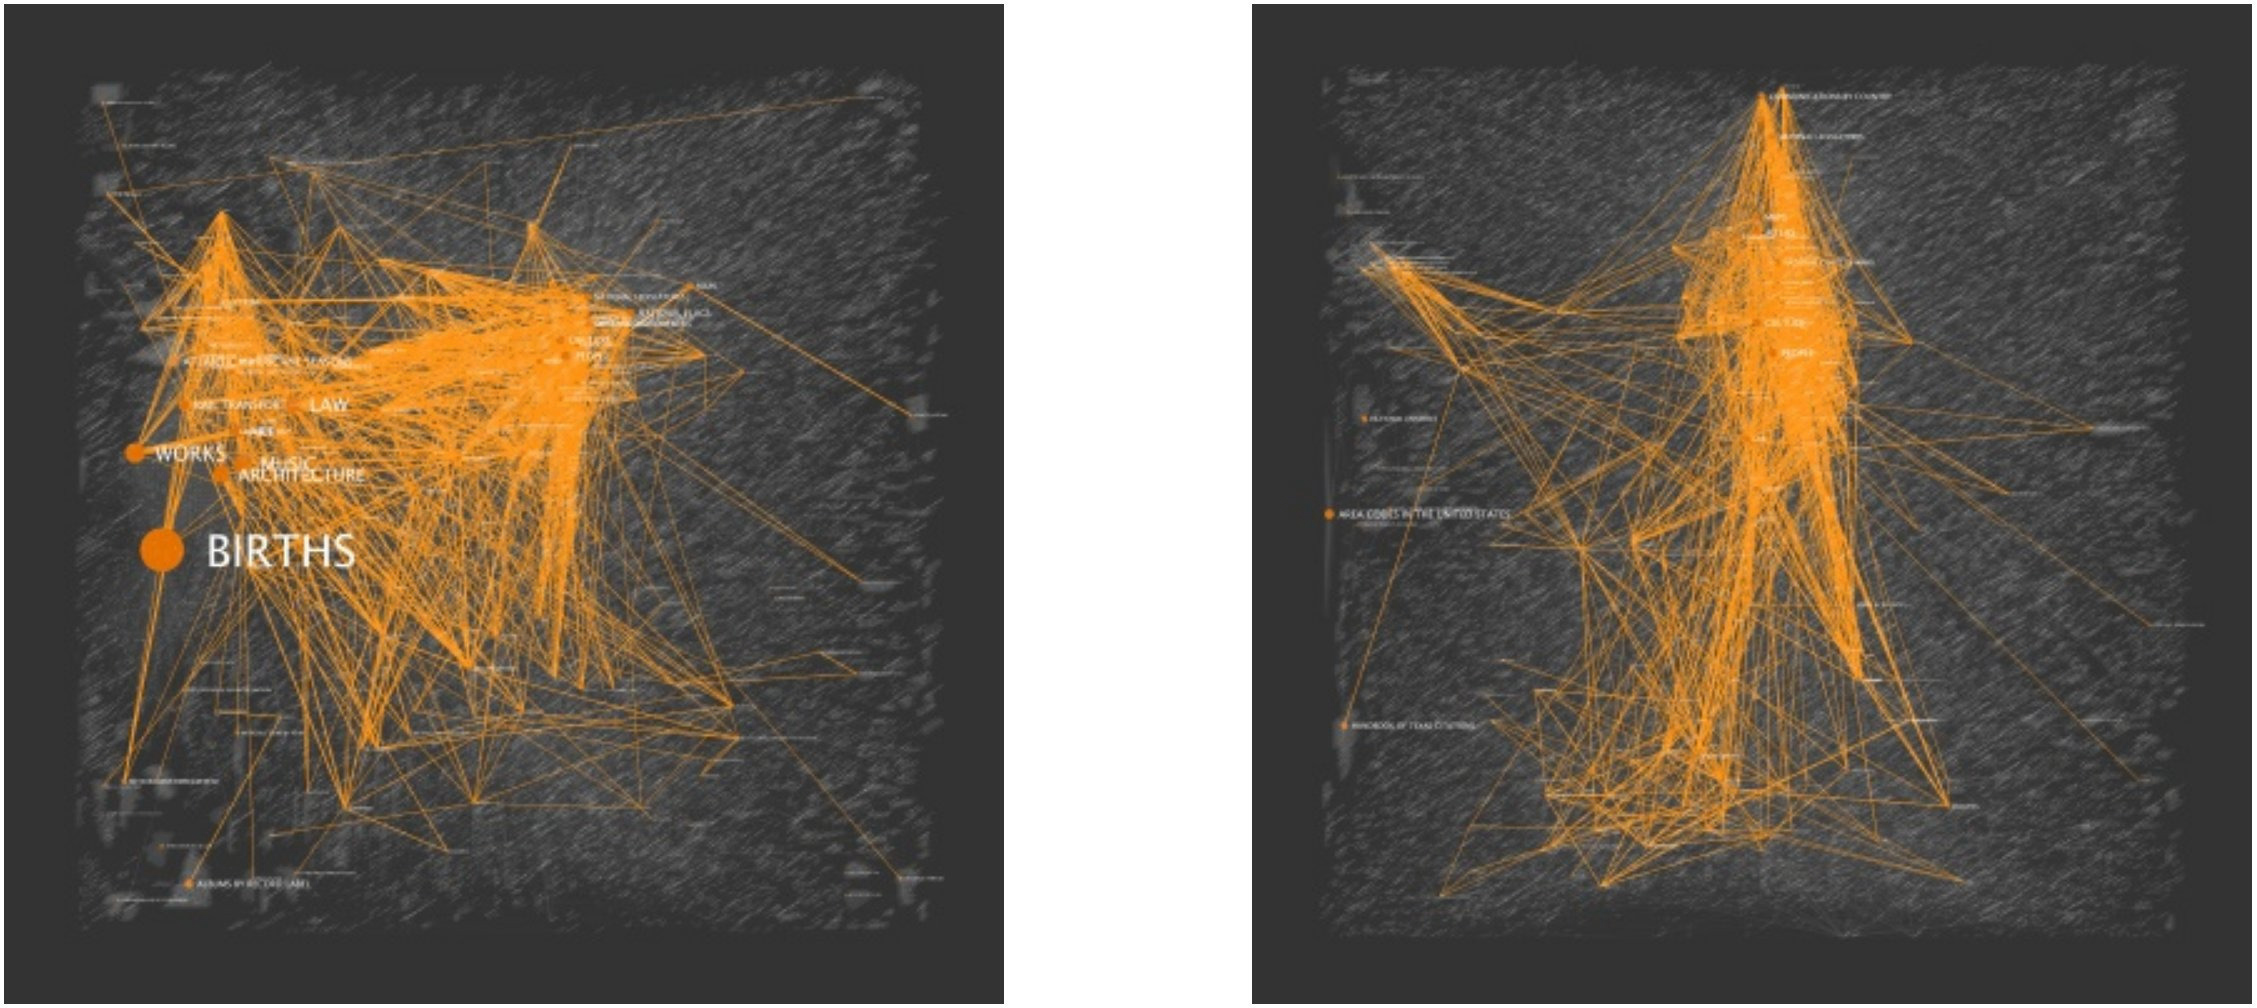
\includegraphics[width=\textwidth]{images/har-wikiviz}
    \caption{WikiViz \cite{harrison2006wikiviz}}
    \label{fig:harr-wikiviz}
\end{figure}
Auf ähnliche Weise wie Holloway behandelt die Arbeit von Biuk-Aghai~\cite{biuk2011wikipedia} die inhaltliche Reichweite der Wikipedia.
Die Anordnung der Daten erfolgt bei Biuk-Aghai entsprechend dem \emph{Radial Convergence Model} nach Lima~\cite[S.~63]{lima2017circle}.
Die Visualisierung übersetzt die Größe der \emph{Top-Level}-Kategorien anhand der Anzahl der enthaltenen Artikel in einen Balken auf dem äußeren Ring. Vertiefend werden die direkten Unterkategorien mit ihren Titeln weiter außen im Ring gezeichnet, um die \emph{Top-Level} Kategorien detailreicher zu umschreiben.
Innerhalb des Rings werden alle Artikel als Knoten dargestellt, wobei die Position eines Knotens von der Ähnlichkeit des zugehörigen Artikels zu den Kategorien abhängig ist.
% Die Arbeit von Picandet \cite{picandet2014wikiabout} versucht auf die selbe art die 


In der Arbeit \emph{ClusterBall} von Harrison~\cite{harrison2006clusterbal} werden Wikipedia-Kategorien in einem \emph{Radial Convergence Model}~ \cite[S.~63]{lima2017circle} angeordnet.
Im Fokus der Visualisierung steht die Bildung und Darstellung von \emph{Kategorienclustern}.
Infolgedessen werden die Kategorien in drei unterschiedliche Gruppen eingeteilt: Erstens eine Startkategorie im Zentrum der Darstellung, zweitens Kategorien auf dem äußeren Ring und drittens solche Kategorien, die sich innerhalb des Ringes befinden.
Die Kanten bilden die Verbindungen zwischen den Kategorien ab und sind, je nach ihrer Gruppenzugehörigkeit, unterschiedlich gefärbt.
Die Kategorien auf dem äußeren Ring werden so angeordnet, dass die Kantenlänge minimiert wird, was wiederum zu einer eindeutig erkennbaren Bildung von \emph{Clustern} führt.
Die Kategorien innerhalb des Rings, in der Abbildung~\ref{fig:harr-cluster} als blaue Knoten zu erkennen, bilden ein \emph{Cluster}. 

\begin{figure}[H]
    \centering
    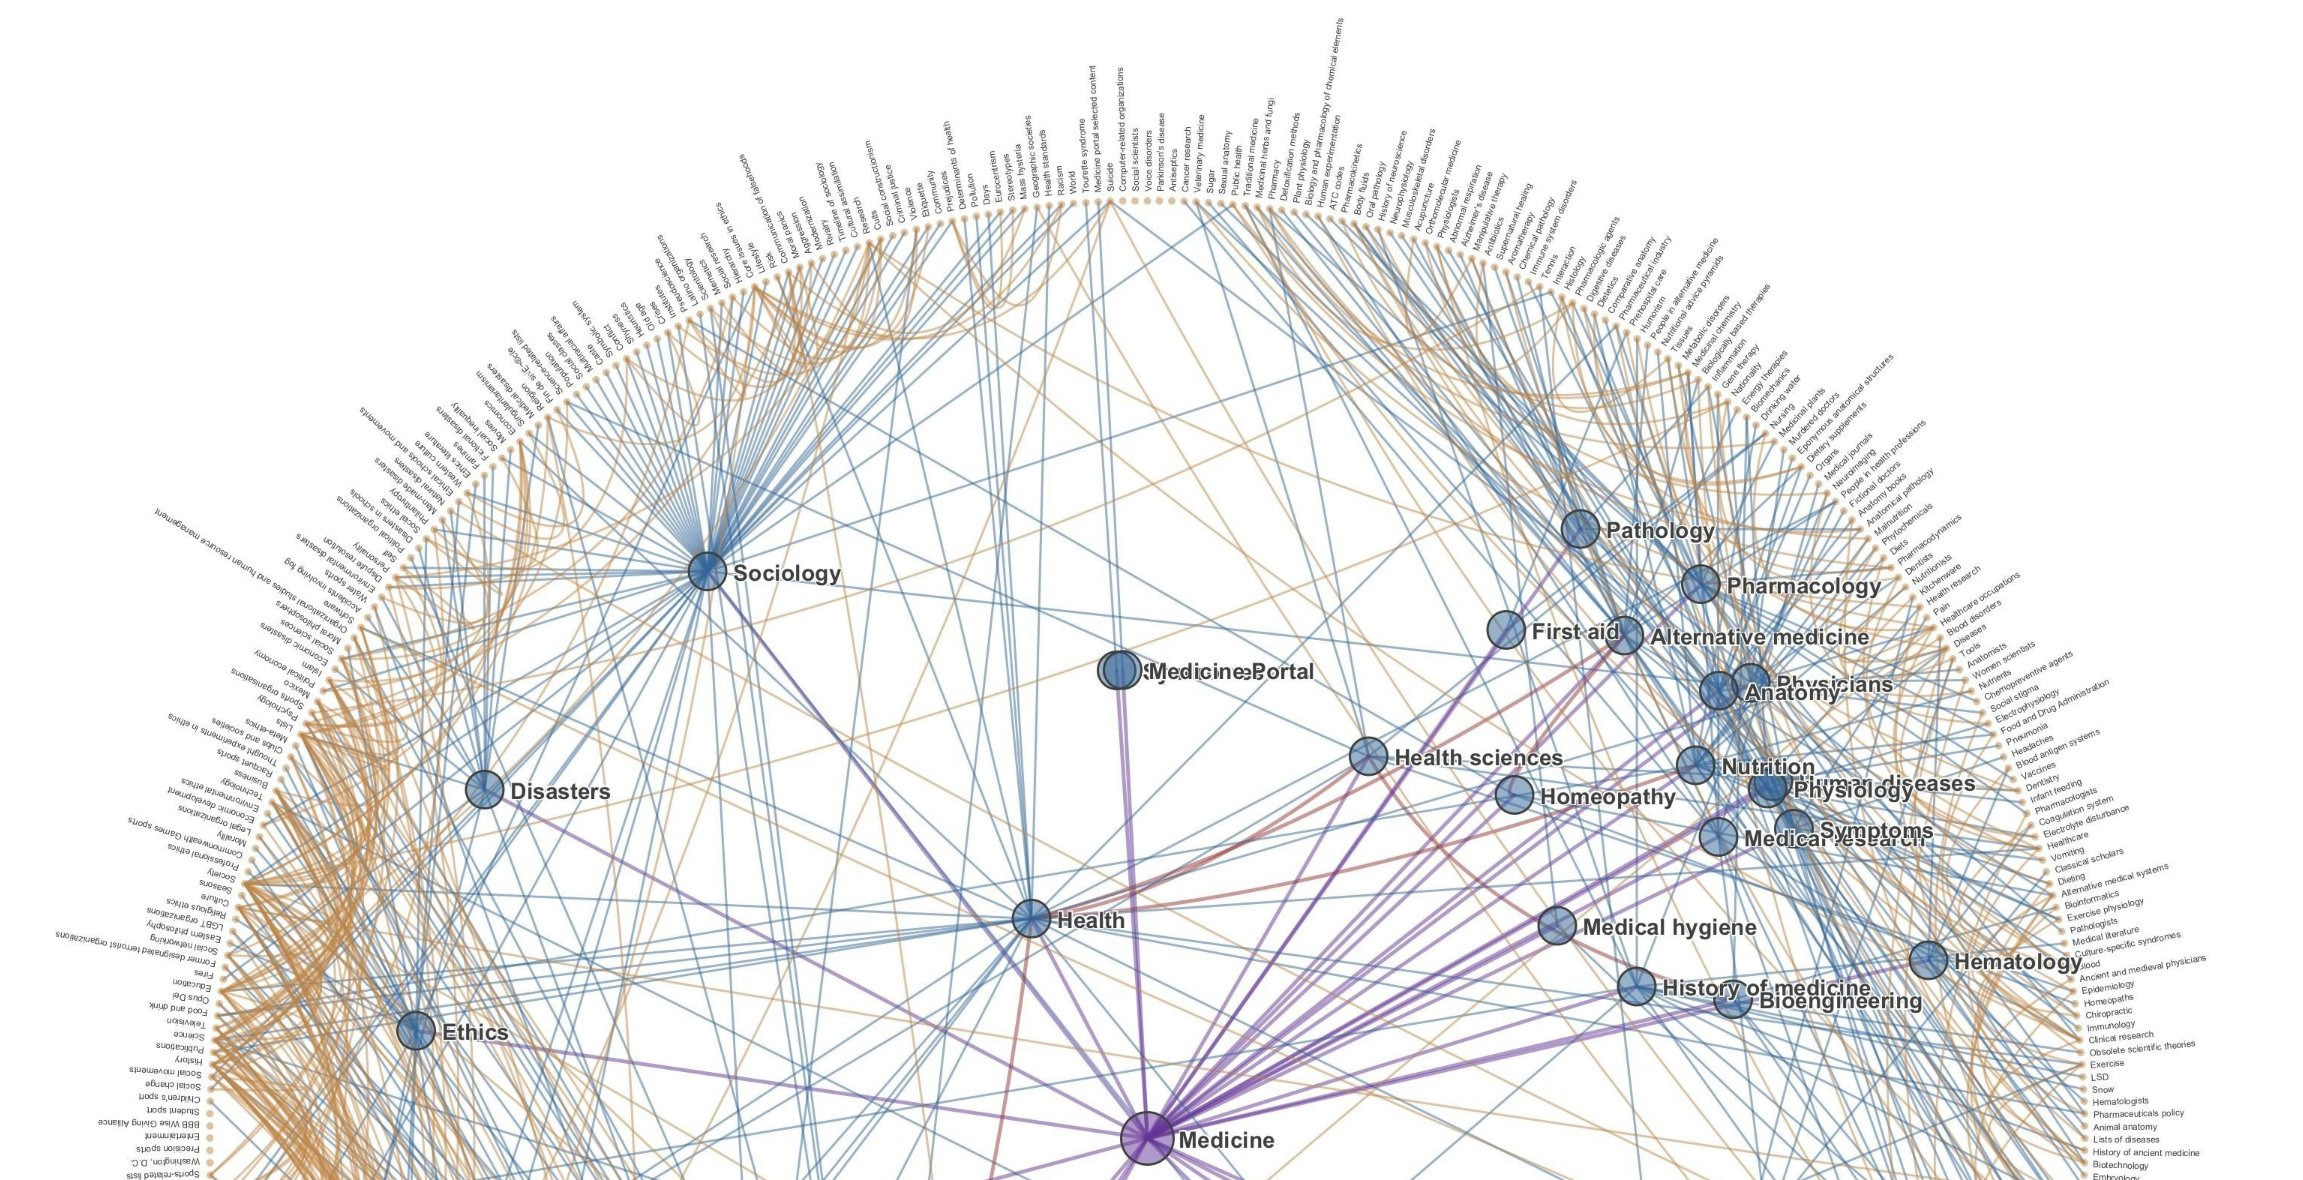
\includegraphics[width=\textwidth]{images/clusterball}
    \caption{Clusterball \cite{harrison2006clusterbal}}
    \label{fig:harr-cluster}
\end{figure}

Die Visualisierung von Clever~\cite[S.~233]{lima2017circle} stellt die Hierarchie des Kategoriensystems der Nationalbibliothek der Niederlande dar.
Auch Clever verwendet eine radial angeordnete hierarchische Struktur.
Seine Visualisierung unterscheidet jedoch farblich nicht zwischen Kategorien der ersten Ebene und Kategorien niedrigerer Ebenen.
Die Herangehensweise von Clever, die Kategorienhierarchie zur Ordnung und Suche in Archiven zu nutzen, liefert einen Impuls für die vorliegende Arbeit.



% \section{Graphen und B"aume}
% MoireGraphs: Radial Focus+Context Visualization and Interaction for Graphs with Visual Nodes \cite{jankun2003moiregraphs}
% RINGS : A Technique for Visualizing Large Hierarchies \cite{teoh2002rings}
% Visualization of Large Hierarchical Data by Circle Packing \cite{wang2006circlepacking}

% \section{Radiales Layout}

% A parent-centered radial layout algorithm for interactive graph visualization \cite{pavlo2006parent}





